\documentclass[a4paper, 11pt, final, garamond]{book}
\usepackage{cours-preambule}

\raggedbottom

\makeatletter
\renewcommand{\@chapapp}{Travaux pratiques -- TP}
\makeatother

\let\SavedIndent\indent
\protected\def\indent{%
  \begingroup
    \parindent=\the\parindent
    \SavedIndent
  \endgroup
}
\setlength{\parindent}{0pt}

\begin{document}
\setcounter{chapter}{7}

\chapter{Oscillateurs amortis en \'electricit\'e et m\'ecanique}
\section{Objectifs}

\begin{itemize}
    \item Étudier plus précisément le régime pseudo-périodique d'un circuit RLC
        peu amorti.
    \item  Étudier le comportement d'un oscillateur mécanique vertical amorti
        avec amortissement faible.
    \item  Tracer  une allure de trajectoire de phase correspondant au régime
        pseudo-périodique.
    \item  Vérifier la décroissance exponentielle des amplitudes dans les deux
        domaines.
    \item  Établir un tableau des analogies entre la mécanique et l'électricité.
\end{itemize}


\section{S'approprier}

%\subsection{Définition générale d'une trajectoire de phase (hors-programme)}
%
%Définition~: On peut décrire l'évolution d'un système quelconque (mécanique ou électrique), pour des conditions initiales données, par la trajectoire dans l'\textbf{espace des phases} $(x \, ; \dot{x})$  ou $(u_{C} \, ; \dot{u_{C}})$ ou  plus généralement (variable~; dérivée de la variable) appelée \textbf{trajectoire de phase}. L'ensemble des trajectoires de phase, pour toutes les conditions initiales possibles, est appelé \textbf{portrait de phase}. 

\subsection{Rappel concernant l'oscillateur mécanique vertical}

\begin{wrapfigure}[11]{r}{0.60\linewidth}
    \vspace{-35pt}
    \begin{center}
        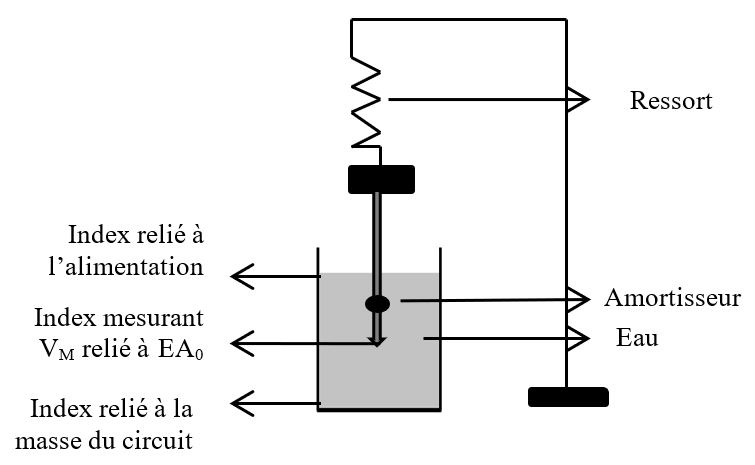
\includegraphics[width=0.55\textwidth]{OH}
    \end{center}
\end{wrapfigure} 

Soit un oscillateur mécanique vertical (cf.\ figure ci-contre), constitué d'un
ressort de raideur $k = \SI{10}{N.m^{-1}}$ et d'une masse $m = \SI{200}{g}$. Il
est légèrement amorti par frottement fluide dans l'air, caractérisé par une
force de la forme~: $\vect{f}= - \lambda\vect{v}$. 

\medskip

Dans ce cas, l'équation différentielle (obtenue par projection selon la direction verticale $z$ du PFD) de l'oscillateur harmonique amorti peut se mettre sous la forme~:

\centers{$\DS\ddot{z} + \frac{\lambda}{m} \dot{z} + \frac{k}{m} z = 0$}

\underline{Remarque}~: $z$ est une variable bien choisie pour qu'on ait à
l'équilibre $z=0$. C'est la raison pour laquelle le poids ainsi que la longueur
à vide du ressort n'apparaissent pas explicitement dans l'expression. 

\section{Analyser~: régime pseudo-périodique du RLC série}

\begin{enumerate}
    \item Faire le schéma d'un circuit RLC série alimenté par une tension
        $e(t)$. On veut visualiser à l'oscilloscope simultanément $e(t)$ sur la
        voie 1 et $u_{C}(t)$ sur la voie 2. Indiquer les connexions de
        l'oscilloscope à réaliser et positionner la masse sur le circuit.

    \item $e(t)$ est une tension créneau de fréquence $\SI{100}{Hz}$, $C$ une
        boite de capacités. On prendra $C = \SI{0,01}{\micro F}$. $L$ est une
        bobine d'inductance $L= \SI{0,1}{H}$. Écrire l'équation différentielle
        en $u_{C}(t)$, puis celle en $q(t) = C u_{C}(t)$ et calculer la valeur
        $R_{c}$ à donner à $R$ pour visualiser le régime critique.
\end{enumerate}

\section{Réaliser et valider}

\subsection{Étude expérimentale du régime pseudo-périodique du circuit RLC}

Réaliser le montage vu précédemment dans l'analyse en prenant les mêmes valeurs
de $e(t)$, $C$ et $L$ que ci-dessus.

\textbf{a  -- Visualisation du régime pseudo-périodique et mesure de la
pseudo-période}~:

\begin{enumerate}
    \item Faire varier $R$ de façon à observer un régime pseudo-périodique très
        peu amorti~: Il faut observer au moins une dizaine de maxima successifs
        sur l'oscillogramme.
    \item Dans le cas d'un amortissement très faible, on peut assimiler la
        pseudo-période des oscillations $T$ à la période propre $T_0$ du
        circuit. Mesurer expérimentalement la pseudo-période $T$ en prenant
        plusieurs périodes pour gagner en précision et la comparer à la période
        propre théorique en calculant l'écart relatif entre les deux grandeurs.
    \item Imprimer la courbe obtenue en tenant compte des consignes indiquées
        sur les fiches plastifiées.
\end{enumerate}

\textbf{
    b -- Vérification de la décroissance exponentielle de l'amplitude des
oscillations}~:

\begin{enumerate}
    \item Grâce au curseur horizontal de l'oscilloscope, relever les valeurs des
        amplitudes successives $U_{C,\max}$ en fonction du nombre de périodes
        $nT$.

    \item Ouvrir \texttt{latispro} (programmes $\rightarrow$ discipline
        $\rightarrow$ physique-chimie $\rightarrow$ eurosmart $\rightarrow$
        latispro), puis générer le tableau de valeurs $(nT \, ; \, U_{C,\max})$
        correspondant. Créer ensuite la variable nécessaire de façon à vérifier
        que l'amplitude des oscillations décroit de façon exponentielle. On
        cherchera à faire une modélisation par une droite. Relever alors le
        coefficient directeur $a_{\exp}$ de la droite obtenue. Le comparer (en
        calculant l'écart relatif par exemple) à la valeur théorique $a_{\rm
        theo}$ attendue (en fonction de $R$, $C$ et $L$) que vous expliciterez.
        Imprimer la courbe obtenue ainsi que sa modélisation. Quel est le lien
        entre le coefficient directeur $a$ et le décrément logarithmique
        introduit dans le TD~? 
\end{enumerate}

\subsection{Étude expérimentale d'oscillations mécaniques amorties}

\textbf{a -- Montage expérimental}~:

Le montage est schématisé dans la partie S'approprier et est déjà réalisé. La
masse $m$ ne doit pas toucher à l'eau de l'éprouvette.

\textbf{b -- Réglages de l'ordinateur}~:

Avant tout réglage~: brancher l'interface SYSAM et l'alimentation stabilisée sur
$\SI{7}{V}$.

Ouvrir latispro (programmes $\rightarrow$ discipline $\rightarrow$
physique-chimie $\rightarrow$ eurosmart $\rightarrow$ latispro).

\medskip

Pour faire une acquisition~: bouton

\includegraphics[width=0.05\textwidth]{bouton_acq}

\medskip

Pour activer la voie $EA0$~:

\begin{itemize}
    \item Dans le cadre \textit{entrées analogiques}, cliquer sur  les boutons
        des entrées à activer.
    \item Cliquer droit et choisir \textit{trait}.
\end{itemize}

Pour paramétrer l'acquisition~:

\begin{itemize}
    \item Dans le cadre acquisition, onglet temporel, mode normal, entrer le
        nombre de points de mesure et la durée totale de l'acquisition.
    \item Acquisition temporelle~; durée~: $\SI{30}{s}$~; nombre de points~:
        2000.
\end{itemize}

Fin des réglages~! Vous êtes prêtz à faire vos enregistrements~: on mesure une
tension sur la voie $EA0$ qui est proportionnelle à l'abscisse $z$ du point
matériel de masse $m$.

\textbf{c - Mesures}~:

\begin{itemize}
    \item Lorsque la position est à sa position d'équilibre, le bout du fil doit
        être au milieu du bécher. Si ce n'est pas le cas, modifier la hauteur du
        point d'attache du ressort. 
    \item Étirer légèrement le ressort sans qu'il ne touche au fond du bécher. 
    \item Lorsque les oscillations paraissent régulières, lancer l'acquisition
        en cliquant sur 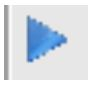
\includegraphics[width=0.05\textwidth]{bouton_go}.
\end{itemize}

\textbf{d  -- Exploitation des résultats}~:

\medskip

\underline{Mesure de la pseudo-période des oscillations}~:

Dans le cas d'un amortissement très faible, on peut assimiler la pseudo-période des oscillations $T$ à la période propre $T_0$ du circuit. Grâce au réticule (cliquer droit et choisir),  mesurer expérimentalement la pseudo-période $T$ en prenant plusieurs périodes pour gagner en précision et la comparer à la période propre théorique en calculant l'écart relatif entre les deux grandeurs.

\medskip

\underline{Vérification de la décroissance exponentielle de l'amplitude des
oscillations}~:

\begin{itemize}
    \item Grâce au réticule (lié à la courbe pour plus de facilité), relever les
        valeurs des amplitudes successives $U_{\max}$ en fonction du nombre de
        périodes $nT$ (environ 15 mesures)~; cliquer droit, puis calibrage pour
        modifier l'échelle.
    \item Puis créer le tableau de valeurs $(nT~; U_{\max})$ correspondant, et
        créer la variable nécessaire de façon à vérifier que les amplitudes des
        oscillations décroit de façon exponentielle. On cherchera à faire une
        modélisation par une droite. Relever alors le coefficient directeur
        $a_{\exp}$ de la droite obtenue. Grâce aux relations vues en cours, en
        déduire un ordre de grandeur du coefficient d'amortissement $\lambda$.
        Imprimer la courbe obtenue ainsi que sa modélisation.
\end{itemize}

%\medskip
%
%\underline{Tracé d'une trajectoire de phase}~:
%
%\begin{itemize}
%\item Créer la variable dérivée nécessaire au tracé de la trajectoire de phase~: $deriv(EA0 \, ; \, t)$~: dérivée du signal de la voie $EA0$ par rapport au temps $t$.
%\item Tracer la trajectoire de phase grâce aux choix d'abscisses et d'ordonnées dans les options de graphe. Imprimer la courbe. Quelle est l'allure de la courbe obtenue~? Commenter qualitativement. Intuiter l'allure s'il n'y avait aucun amortissement. 
%\end{itemize}

\section{Conclure}

Quelles similitudes de comportements entre les deux types d'oscillateurs ont été
observées~? En utilisant les études théoriques demandées (équations
différentielles), ainsi que les résultats expérimentaux trouvés, recopier et
compléter le tableau suivant~:

\begin{center}
    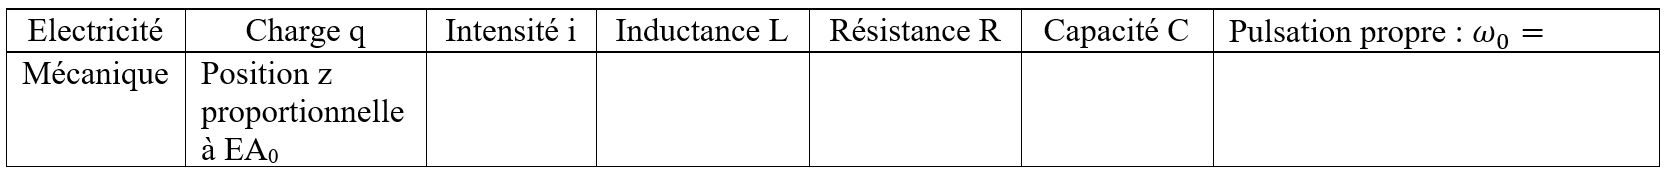
\includegraphics[width=\textwidth]{tab}
\end{center}
  
\end{document}
